\subsection{Использование АР для детектирования ШПС}
Известно, что АР подход широко применяется в детектировании и кодировании голоса и видео, в восстановлении сигналов и т.д.
Более точно - АР-модели целесообразно применять для получения спектров с острыми пиками, но без глубоких впадин (нулей).
Так же в пользу выбора АР-модели может быть принят тот факт, что часто вычислительные затраты для оценивания АР-модели 
ниже чем вычислительные затраты требуемые для оценки параметров СС- и АРСС моделей \cite{marpl_book}.

Специфичной для детектирования ШПС является необходимость определения точной фазы ПСП
для работы с сигналом. Так же при обработке ШПС от нескольких источников с разными ПСП необходимо учитывать,
что оценка спектра будет смещенной и требуется его корректировка. Следует учитывать, что после демодуляции
с синхронизированной копией ПСП получается гармоничнская компонента и шум. Подробнее компоненты шума были
рассмотрены в \ref{l:noise_model}. Преобразуем выражение \ref{eq:gps_signal_modulated}: амплитуду гармонического
сигнала возьмем ${\sqrt{2A} = 1}$, ${D_k(t)}$ примем за 1, учитывая, что мы детектируем сигнал в пределах одного
информационного бита:
\begin{center}
\begin{equation}
	\label{eq:lpc_signal}
	s(t) = \cos(\omega_{c}t) + n(t)
\end{equation}
\end{center}

Для применения АР метода является очень существенным знать модель шумовой компоненты из ${n(t)}$ из выражения
\ref{eq:lpc_signal}. Зная АКФ ${n(t)}$, можно получить несмещенную оценки ${\omega_c}$.

\subsubsection{Детектирование ШПС от одного источника}

Рассмотрим простейший случай - применение данного подхода для детектирования одного сигнала ШПС.
Схема алгоритма представлена на рисунке \ref{pic:lpc_basic}

\begin{figure}[H]
	\center\scalebox{0.8}{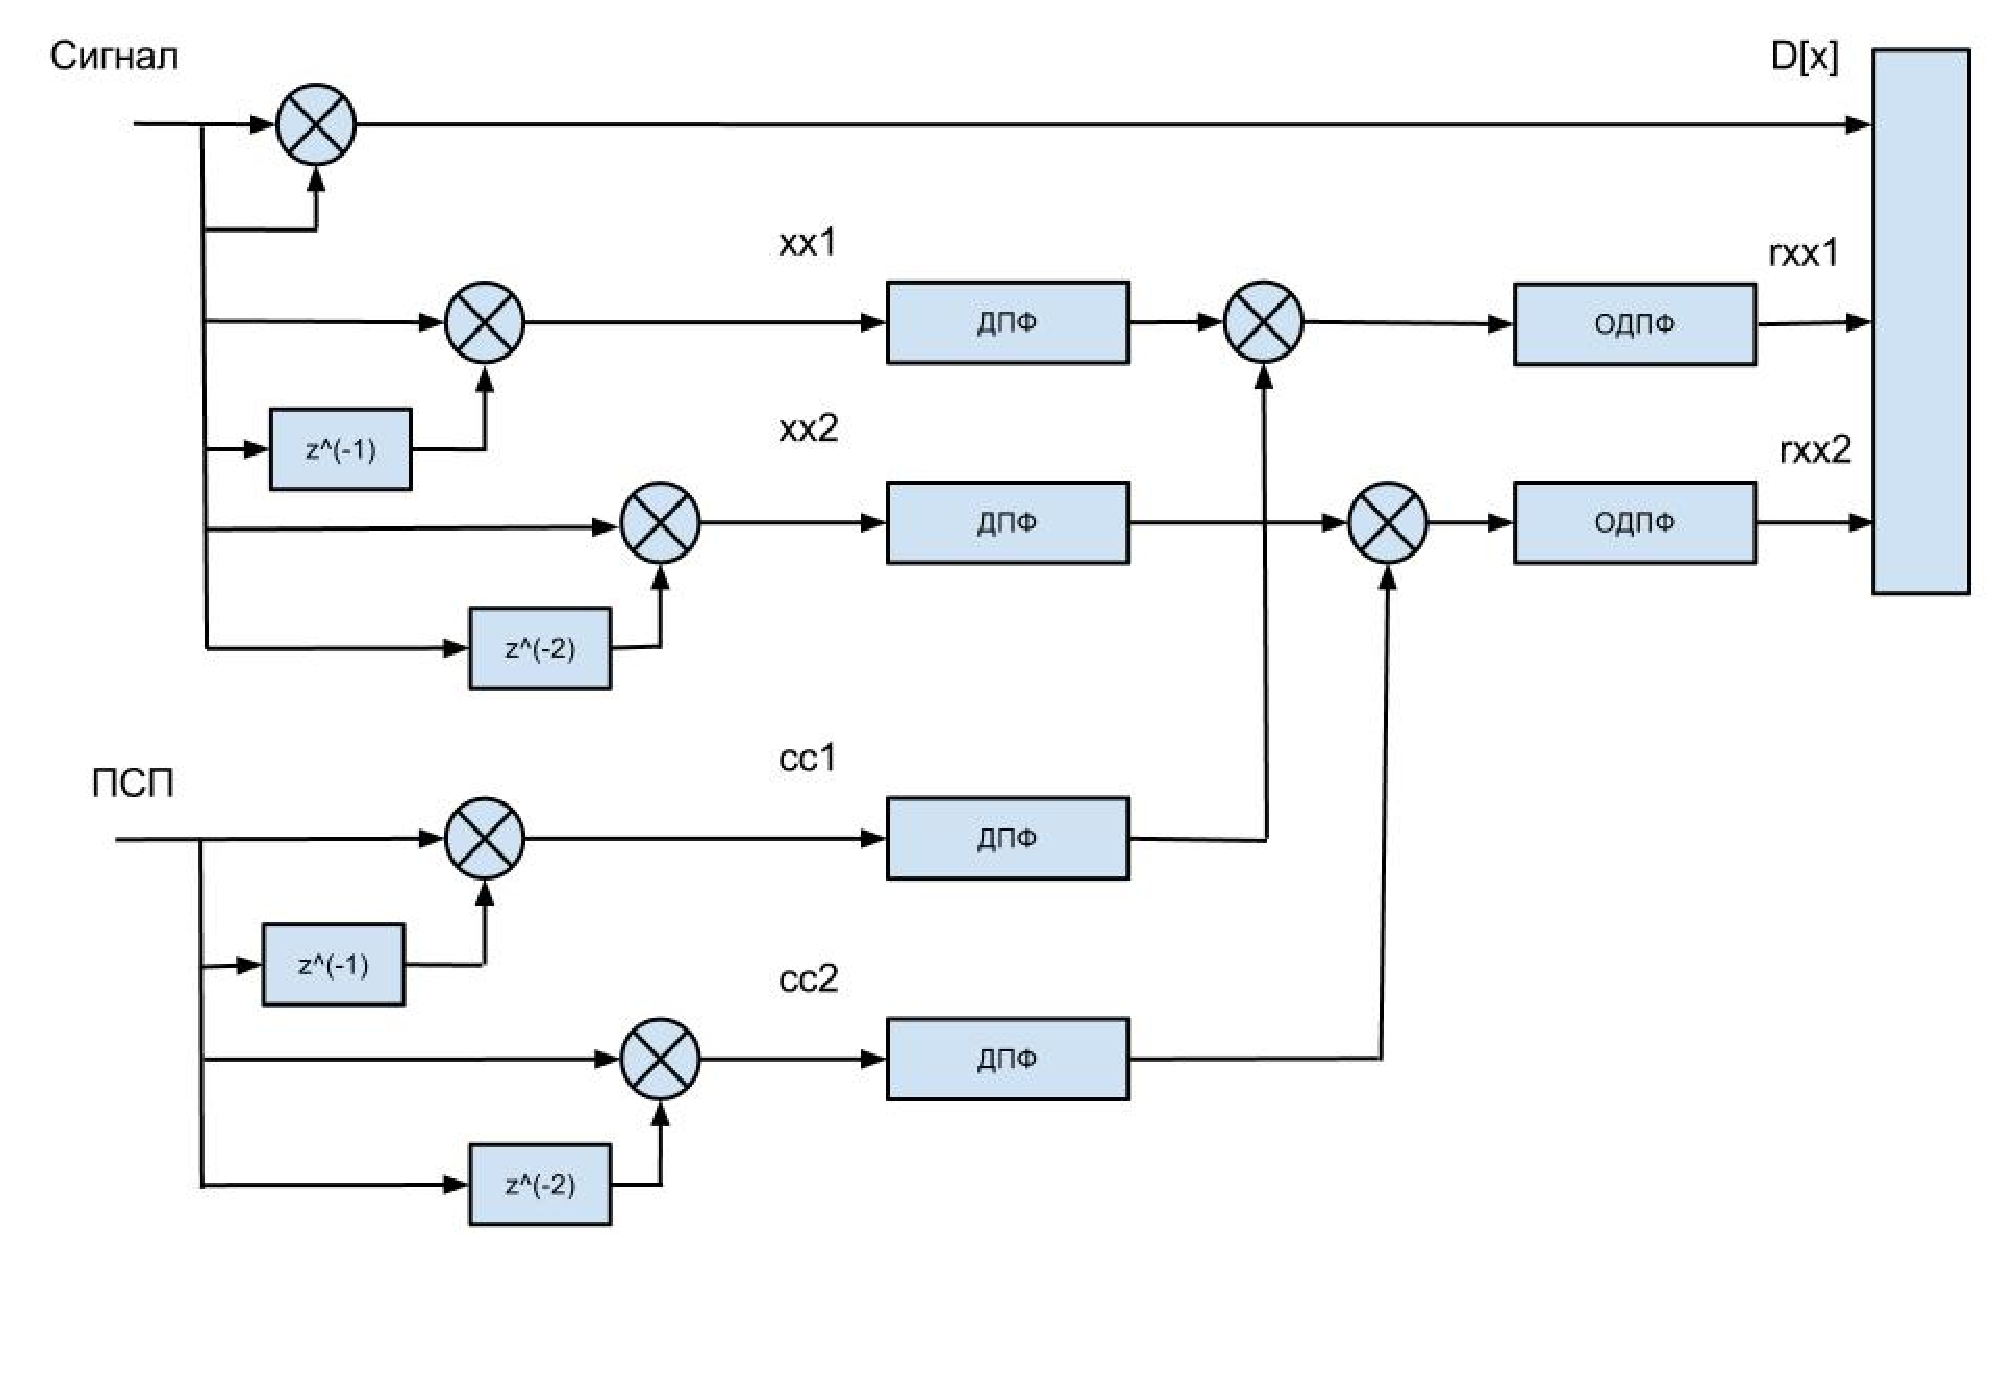
\includegraphics[width=1\linewidth]{lpc.eps}}
	\caption{Общая схема применения АР модели для детектирования ШПС сигнала}
	\label{pic:lpc_basic}
\end{figure}
Для перебора фаз ПСП воспользуемся БПФ, в результате получим значения корреляции для каждой фазы ПСП (глава \ref{sec1_fft}).
Поскольку демодуляция ПСП восстанавливает единственную гармоническую компоненту, необходимо искать 1 частоту - 1 полюс.
Тогда выражение \ref{eq:lpc_rms2} может быть записано как:
\begin{center}
\begin{equation}
	\label{eq:lpc_gps_1}
	{\bf a} = 
		\left[ \begin{array}{cc}
			r_{xx}(0) & r_{xx}(1) \\
			r_{xx}(1) & r_{xx}(0)
		\end{array} \right]
		\left[ \begin{array}{c}
			r_{xx}(1) \\
			r_{xx}(2)
		\end{array} \right]
\end{equation}
\end{center}

Выражение \ref{eq:lpc_gps_1} не учитывает коррекцию. Это будет рассмотрено позднее. После получения коэффициентов АР модели
${\bf{a}}$ можно построить график оценки СПМ для смещения, содержащего максимальный спектральный пик - гармоническую компоненту
с наивысшей энергией - рисунок \ref{pic:lpc_psd_1} и график состоящий из максимальных спектральных пиков для каждой фазы
ПСП - рисунок \ref{pic:lpc_1sat_energy}.

\begin{figure}[H]
	\center\scalebox{1}{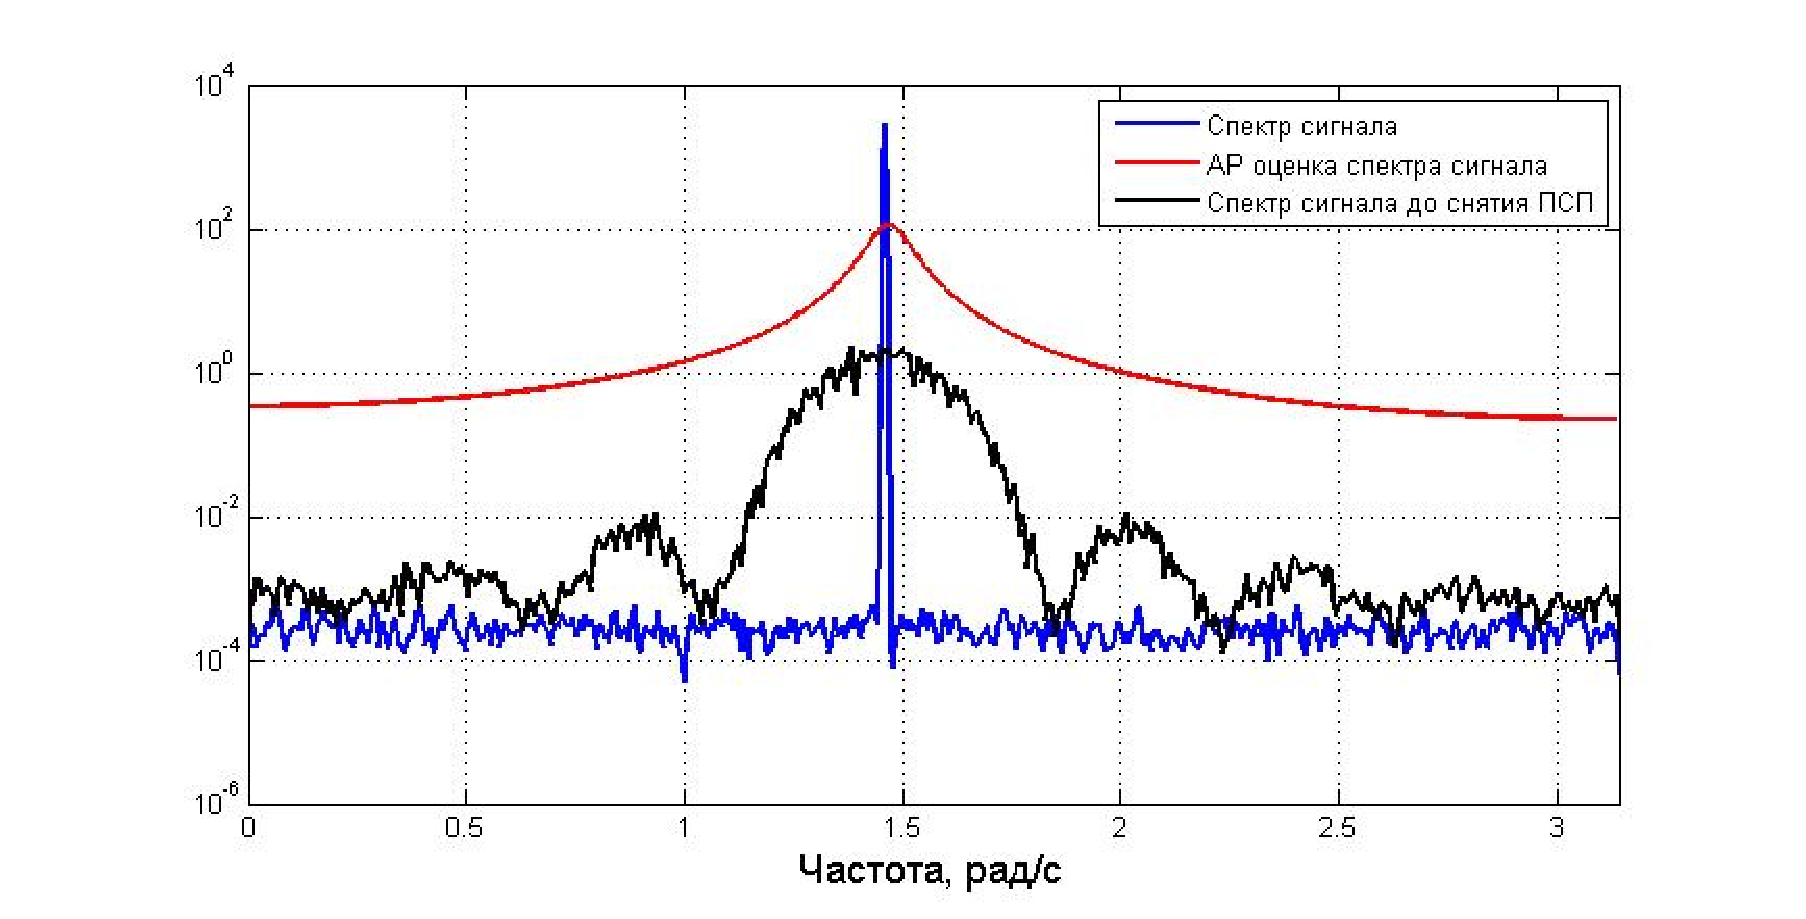
\includegraphics[width=1\linewidth]{lpc_1sat.eps}}
	\caption{Оценка СПМ сигнала модулированного ПСП}
	\label{pic:lpc_psd_1}
\end{figure}
\begin{figure}[H]
	\center\scalebox{1}{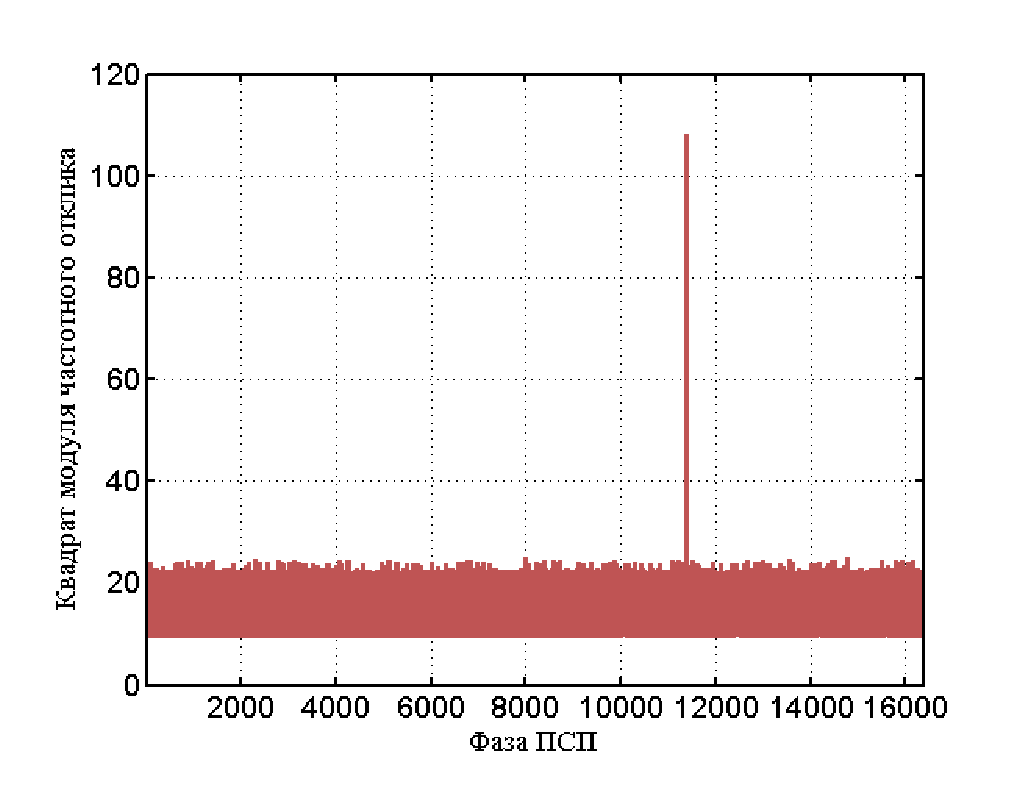
\includegraphics[width=1\linewidth]{lpc_1sat_energy.eps}}
	\caption{Максимальыне пики для каждой фазы ПСП}
	\label{pic:lpc_1sat_energy}
\end{figure}

Но любой шум, отличный АБГШ будет смещать оценку частоты. На рисунке \ref{pic:lpc_1sat_interference}
представлен график смещения оценки в зависимости от мощности второго луча сигнала, модулированного
той же ПСП.

\begin{figure}[H]
	\center\scalebox{1}{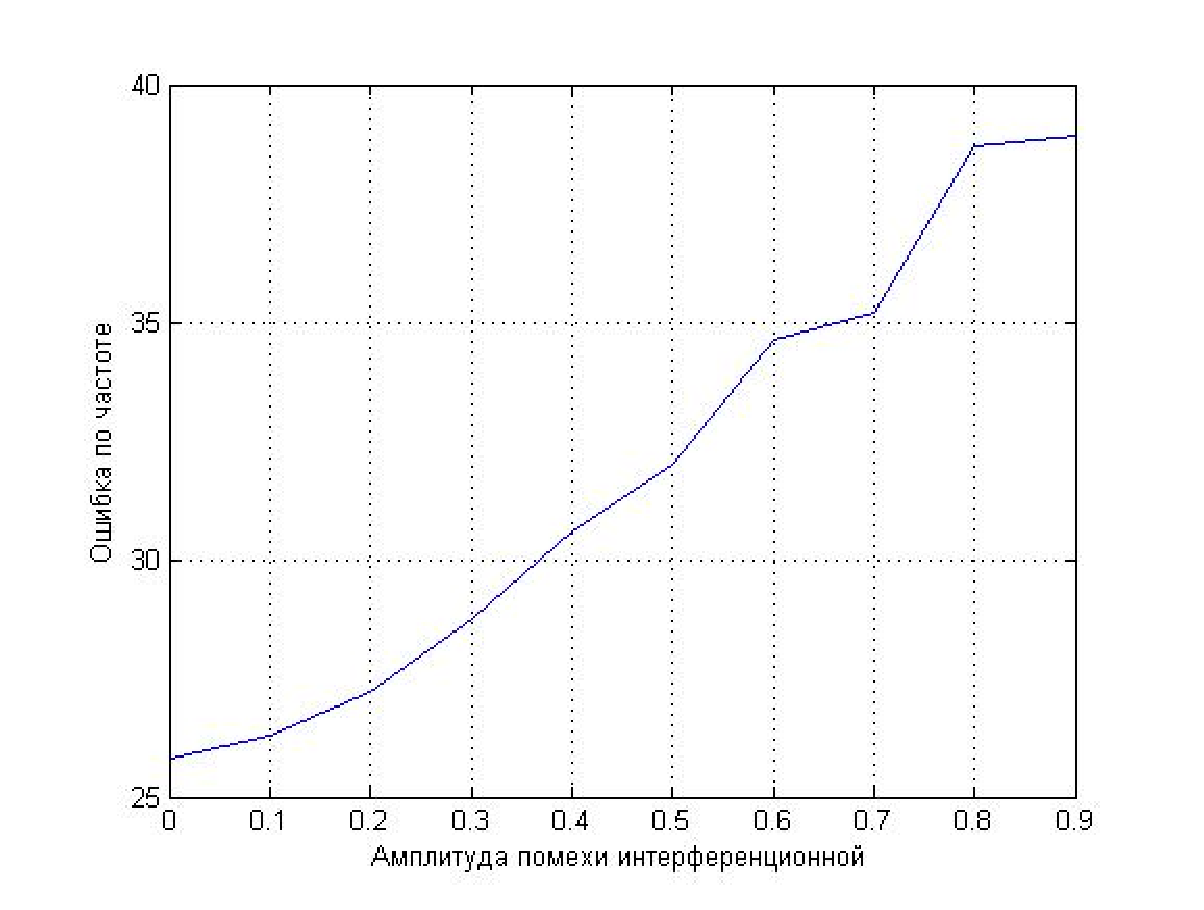
\includegraphics[width=1\linewidth]{lpc_interference.eps}}
	\caption{Зависимость ошибки оценки пика от энергии интерференционной помехи}
	\label{pic:lpc_1sat_interference}
\end{figure}

%%%%%%%%%%%%%%%%%%%%%%%%%%%%%%%%%%%%%%%%%%%%%%%
\subsubsection{Детектирование ШПС с коррекцией шума}

\begin{center}
\begin{equation}
	\label{eq:lpc_gps_1}
	{\bf a} = 
		\left(
			\left[ \begin{array}{cc}
				r_{xx}(0) & r_{xx}(1) \\
				r_{xx}(1) & r_{xx}(0)
			\end{array} \right] -
			\left[ \begin{array}{cc}
				\sigma & 0 \\
				0 & \sigma
			\end{array} \right] 
		\right)
		\left[ \begin{array}{c}
			r_{xx}(1) \\
			r_{xx}(2)
		\end{array} \right]
\end{equation}

\end{center}
\newpage
